% SPDX-License-Identifier: CC-BY-NC-SA-3.0

% Copyright 2022 KUNBUS GmbH
% With work from https://git-scm.com/book/en/v2

\documentclass[aspectratio=169]{beamer}

\usepackage{minted}
\usepackage{xcolor}
\definecolor{LightGray}{gray}{0.9}

\usetheme {default}
\setbeamertemplate{navigation symbols}{}

\graphicspath{{images/}{\main/images/}}

% Title page details
\title {git training\footnote{This work is licensed under a \href{http://creativecommons.org/licenses/by-nc-sa/3.0/}{Creative Commons Attribution-NonCommercial-ShareAlike 3.0 Unported License.}}}
\subtitle{git, workflows, github}
\author{Philipp Rosenberger}
\institute{KUNBUS GmbH}
%\date{\today}

\renewcommand{\footnotesize}{\tiny}

\newcommand{\sectiontitle}{}
\newcommand{\newsection}[1]{\renewcommand{\sectiontitle}{#1}\section{#1}}

% Image Logo
\logo{\includegraphics[width=2.5cm]{kunbus-logo.png}} 

\begin{document}

\begin{frame}
% Print the title page as the first slide
\titlepage
\end{frame}

% Presentation outline
\begin{frame}{Outline}
    \tableofcontents
\end{frame}

\section{What is a VCS?}
\begin{frame}{What is a VCS?}
\begin{itemize}
    \item Tracks changes
    \item Creates a history over the changes
    \item Provides traceability
    \item Provides attribution
\end{itemize}
\end{frame}

\begin{frame}{Centralized VCS}{Centralized vs. Distributed VCS}
\begin{figure}
    \centering
    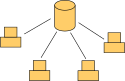
\includegraphics[width=\textwidth,height=0.6\textheight,keepaspectratio]{01_centralized_vcs}
\end{figure}
\end{frame}

\begin{frame}{Distributed VCS}{Centralized vs. Distributed VCS}
\begin{figure}
    \centering
    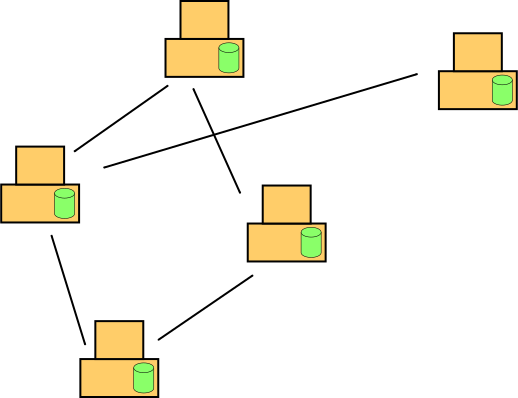
\includegraphics[width=\textwidth,height=0.6\textheight,keepaspectratio]{02_distributed_vcs}
\end{figure}
\end{frame}

\begin{frame}{Deltas}{Deltas vs. Snapshots}
\begin{figure}
    \centering
    \includegraphics[width=\textwidth,height=0.6\textheight,keepaspectratio]{deltas}
    \caption{
        Storing data as changes to a base version of each file\footnote{
            Pro Git: 1.3 Getting Started - What is Git?
            (\url{https://git-scm.com/book/en/v2/Getting-Started-What-is-Git\%3F})
        }
    }
\end{figure}
\end{frame}

\begin{frame}{Snapshots}{Deltas vs. Snapshots}
\begin{figure}
    \centering
    \includegraphics[width=\textwidth,height=0.6\textheight,keepaspectratio]{snapshots}
    \caption {
        Storing data as snapshots of the project over time\footnote{
            Pro Git: 1.3 Getting Started - What is Git?
            (\url{https://git-scm.com/book/en/v2/Getting-Started-What-is-Git\%3F})
        }
    }
\end{figure}
\end{frame}

\section{How does Git work?}
\begin{frame}[fragile]{Every thing is a Hash}{How does Git Work?}
\begin{minted}[bgcolor=LightGray,fontsize=\small]{text}
$ sha1sum kunbus-logo.png 
c263869cf482a5d5d4262170ec242f8f13fc3def  kunbus-logo.png
$ ls -sh kunbus-logo.png 
352K kunbus-logo.png
\end{minted}
\begin{itemize}
    \item A file is an \emph{object} with a \emph{hash} and a \emph{size}
    \item Everything is identified by its hash, not only file objects
\end{itemize}
\end{frame}

\begin{frame}{Git is a Tree of Hashes}{How does Git Work?}
\begin{figure}
    \centering
    \includegraphics[width=\textwidth,height=0.6\textheight,keepaspectratio]{data-model-2}
    \caption{
        The content structure of your current Git data\footnote{
            Pro Git: 10.2 Git Internals - Git Objects
            (\url{https://git-scm.com/book/en/v2/Git-Internals-Git-Objects})
        }
    }
\end{figure}
\end{frame}

\begin{frame}{Git is a Tree of Trees of Hashes}{How does Git Work?}
\begin{figure}
    \centering
    \includegraphics[width=\textwidth,height=0.6\textheight,keepaspectratio]{data-model-3}
    \caption{
        All the reachable objects in your Git directory\footnote{
            Pro Git: 10.2 Git Internals - Git Objects
            (\url{https://git-scm.com/book/en/v2/Git-Internals-Git-Objects})
        }
    }
\end{figure}
\end{frame}

\newsection{Git Basics}
\begin{frame}[fragile]{Getting a Git Repository}{\sectiontitle}
\begin{itemize}
    \item Create a directory
    \item Call \verb|git init| inside the directory
\end{itemize}
\begin{minted}[bgcolor=LightGray,fontsize=\small]{text}
$ mkdir my_project
$ cd my_project
$ git init
Initialized empty Git repository in /home/user/my_project/.git/
\end{minted}
\begin{itemize}
    \item This creates a local repository
    \item It is contained in the \verb|.git| directory under the \verb|my_project| directory
\end{itemize}
\end{frame}

\begin{frame}[fragile]{Getting a Git Repository}{\sectiontitle}
\begin{itemize}
    \item With \verb|git clone| we can get a remote repository
\end{itemize}
\begin{minted}[bgcolor=LightGray,fontsize=\small]{text}
$ git clone https://github.com/libgit2/libgit2
Cloning into 'libgit2'...
remote: Enumerating objects: 119184, done.
remote: Counting objects: 100% (119184/119184), done.
remote: Compressing objects: 100% (32744/32744), done.
remote: Total 119184 (delta 84532), reused 119074 (delta 84433), pack-r...
Receiving objects: 100% (119184/119184), 61.22 MiB | 7.21 MiB/s, done.
Resolving deltas: 100% (84532/84532), done.
\end{minted}
\begin{itemize}
    \item This creates the directory \verb|libgit2|
    \item A git repository (\verb|.git|) is create inside the directory
    \item The git repository contains a \emph{complete} copy of the remote repository
\end{itemize}
\end{frame}

\begin{frame}{Recording Changes to the Repository}{\sectiontitle}
\begin{block}{A file in your working tree can be in one (or more) of these for states}
    \begin{itemize}
        \item unmodified
        \item modified
        \item untracked
        \item staged
    \end{itemize}
\end{block}
\end{frame}

\begin{frame}{Recording Changes to the Repository}{\sectiontitle}
\begin{block}{unmodified}
    Files which are under control of git. All changes have been recorded to the
    history. No additional changes have been made to the files.
\end{block}
\begin{block}{modified}
    Files which are under control of git. Files that have been changed since
    the last time the changes to the file have been recorded to the history.
\end{block}
\end{frame}


\begin{frame}{Recording Changes to the Repository}{\sectiontitle}
\begin{block}{untracked}
    Files which are in the working tree but are not under the control of git.
    They don't exist in the history. This can be new files or build artifacts
    which should not be included in the git repository.
\end{block}
\begin{block}{staged}
    Files which are marked to be recorded to the history. Changes to files files
    in modified stage need to be staged before they can be recorded to the
    history. Also untracked files need to be staged before the can be recorded to
    the history.
\end{block}
\end{frame}

\begin{frame}{Recording Changes to the Repository}{\sectiontitle}
\begin{figure}
    \centering
    \includegraphics[width=\textwidth,height=0.6\textheight,keepaspectratio]{lifecycle}
    \caption{
        The lifecycle of the status of your files\footnote{
            Pro Git: 2.2 Git Basics - Recording Changes to the Repository
            (\url{https://git-scm.com/book/en/v2/Git-Basics-Recording-Changes-to-the-Repository})
        }
    }
\end{figure}
\end{frame}

\begin{frame}[fragile]{Recording Changes to the Repository}{\sectiontitle}
\begin{block}{Example: \ttfamily git add}
\begin{minted}[bgcolor=LightGray,fontsize=\footnotesize,breaklines]{text}
my_project$ echo "# My Project" > README.md
my_project$ git status 
On branch master

No commits yet

Untracked files:
  (use "git add <file>..." to include in what will be committed)
    README.md

nothing added to commit but untracked files present (use "git add" to track)
\end{minted}
\end{block}
\end{frame}

\begin{frame}[fragile]{Recording Changes to the Repository}{\sectiontitle}
\begin{block}{Example: \ttfamily git add}
\begin{minted}[bgcolor=LightGray,fontsize=\footnotesize]{text}
my_project$ git add README.md
my_project$ git status 
On branch master

No commits yet

Changes to be committed:
  (use "git rm --cached <file>..." to unstage)
    new file:   README.md
\end{minted}
\end{block}
\end{frame}

\begin{frame}[fragile]{Recording Changes to the Repository}{\sectiontitle}
\begin{block}{Example: \ttfamily git commit}
\begin{minted}[bgcolor=LightGray,fontsize=\footnotesize]{text}
my_project$ git commit
>EDITOR OPENS<
[master (root-commit) 1945062] Add initial REAMDE.md
 1 file changed, 1 insertion(+)
 create mode 100644 README.md
my_project[master]$ git status 
On branch master
nothing to commit, working tree clean
\end{minted}
\end{block}
\end{frame}

\begin{frame}[fragile]{Recording Changes to the Repository}{\sectiontitle}
\begin{block}{Example: Change file and commit changes}
\begin{minted}[bgcolor=LightGray,fontsize=\footnotesize]{text}
my_project$ echo -e "\nCopyright 2022 KUNBUS GmbH" >> README.md
my_project$ git status
On branch master
Changes not staged for commit:
  (use "git add <file>..." to update what will be committed)
  (use "git restore <file>..." to discard changes in working directory)
    modified:   README.md

no changes added to commit (use "git add" and/or "git commit -a")
my_project$ git add README.md
my_project$ git status 
On branch master
Changes to be committed:
  (use "git restore --staged <file>..." to unstage)
    modified:   README.md
my_project$ git commit
>EDITOR OPENS<
[master c16cceb] Add copyright
 1 file changed, 2 insertions(+)
\end{minted}
\end{block}
\end{frame}

\begin{frame}[fragile]{Recording Changes to the Repository}{\sectiontitle}
\begin{block}{summary}
\begin{itemize}
    \item Add new files with \verb|git add| to the staging area
    \item Add changes with \verb|git add| to the staging area
    \item Use \verb|git status| to check the state of your files and working tree
    \item Use \verb|git commit| to record changes from the staging area to the history
\end{itemize}
\end{block}
\end{frame}

\begin{frame}[fragile]{Viewing the Commit History}{\sectiontitle}
\begin{block}{Example: \ttfamily git log}
\begin{minted}[bgcolor=LightGray,fontsize=\footnotesize]{text}
my_project$ git log
commit c16ccebd91c1a3d4b42cd575ad2912ef671ca506 (HEAD -> master)
Author: Philipp Rosenberger <p.rosenberger@kunbus.com>
Date:   Thu Dec 8 13:15:00 2022 +0100

    Add copyright

commit 19450627f83f4e51ad42ece86d9d2a5279bc2c23
Author: Philipp Rosenberger <p.rosenberger@kunbus.com>
Date:   Wed Dec 7 13:15:11 2022 +0100

    Add initial REAMDE.md
    
    Add a README.md file with just the project name as starting point

\end{minted}
\end{block}
\end{frame}

\begin{frame}[fragile]{Viewing the Commit History}{\sectiontitle}
\begin{block}{Example: \ttfamily git log --pretty=fuller}
\begin{minted}[bgcolor=LightGray,fontsize=\footnotesize]{text}
my_project$ git log --pretty=fuller 
commit c16ccebd91c1a3d4b42cd575ad2912ef671ca506 (HEAD -> master)
Author:     Philipp Rosenberger <p.rosenberger@kunbus.com>
AuthorDate: Thu Dec 8 13:15:00 2022 +0100
Commit:     Philipp Rosenberger <p.rosenberger@kunbus.com>
CommitDate: Thu Dec 8 14:00:34 2022 +0100

    Add copyright

commit 19450627f83f4e51ad42ece86d9d2a5279bc2c23
Author:     Philipp Rosenberger <p.rosenberger@kunbus.com>
AuthorDate: Wed Dec 7 13:15:11 2022 +0100
Commit:     Philipp Rosenberger <p.rosenberger@kunbus.com>
CommitDate: Thu Dec 8 14:00:29 2022 +0100

    Add initial REAMDE.md
    
    Add a README.md file with just the project name as starting point
\end{minted}
\end{block}
\end{frame}

\begin{frame}[fragile]{Viewing the Commit History}{\sectiontitle}
\begin{block}{Example: \ttfamily git show}
\begin{minted}[bgcolor=LightGray,fontsize=\footnotesize]{diff}
my_project$ git show 19450627f83f4e51ad42ece86d9d2a5279bc2c23
commit 19450627f83f4e51ad42ece86d9d2a5279bc2c23
Author: Philipp Rosenberger <p.rosenberger@kunbus.com>
Date:   Wed Dec 7 13:15:11 2022 +0100

    Add initial REAMDE.md
    
    Add a README.md file with just the project name as starting point

diff --git a/README.md b/README.md
new file mode 100644
index 0000000..a2beefd
--- /dev/null
+++ b/README.md
@@ -0,0 +1 @@
+# My Project
\end{minted}
\end{block}
\end{frame}

\begin{frame}[fragile]{Viewing the Commit History}{\sectiontitle}
\begin{block}{summary}
\begin{itemize}
    \item List the history with git \verb|git log|
    \item The difference between author and committer 
    \item Inspect any commit form you history (or git repo) with \verb|git show|
\end{itemize}
\end{block}
\end{frame}

\begin{frame}[fragile]{Undoing Things}{\sectiontitle}
\begin{block}{Example: Change your last commit: \texttt{git commit --amend} {\small(1)}}
\begin{minted}[bgcolor=LightGray,fontsize=\footnotesize]{diff}
my_project$ vim README.md
my_project$ git diff
diff --git a/README.md b/README.md
index 7207d0d..272997d 100644
--- a/README.md
+++ b/README.md
@@ -1,3 +1,3 @@
 # My Project
 
-Copyright 2022 KUNBUS GmbH
+Copyright 2022 KUNBUS GmbH <support@kunbus.com>
my_project$ git status 
On branch master
Changes not staged for commit:
  (use "git add <file>..." to update what will be committed)
  (use "git restore <file>..." to discard changes in working directory)
    modified:   README.md

no changes added to commit (use "git add" and/or "git commit -a")
\end{minted}
\end{block}
\end{frame}

\begin{frame}[fragile]{Undoing Things}{\sectiontitle}
\begin{block}{Example: Change your last commit: \texttt{git commit --amend} {\small(2)}}
\begin{minted}[bgcolor=LightGray,fontsize=\footnotesize]{diff}
my_project$ git add README.md
my_project$ git status 
On branch master
Changes to be committed:
  (use "git restore --staged <file>..." to unstage)
    modified:   README.md

my_project$ git commit --amend
[master 0e59905] Add KUNBUS copyright notice
 Date: Thu Dec 8 13:15:00 2022 +0100
 1 file changed, 2 insertions(+)
\end{minted}
\end{block}
\end{frame}

\begin{frame}[fragile]{Undoing Things}{\sectiontitle}
\begin{block}{Example: Change your last commit: \texttt{git commit --amend} {\small(3)}}
\begin{minted}[bgcolor=LightGray,fontsize=\footnotesize]{diff}
my_project$ git show HEAD
commit 0e59905d83e2d075098d0ea3d0ec4c4f2b45bbfc (HEAD -> master)
Author: Philipp Rosenberger <p.rosenberger@kunbus.com>
Date:   Thu Dec 8 13:15:00 2022 +0100

    Add KUNBUS copyright notice

diff --git a/README.md b/README.md
index a2beefd..272997d 100644
--- a/README.md
+++ b/README.md
@@ -1 +1,3 @@
 # My Project
+
+Copyright 2022 KUNBUS GmbH <support@kunbus.com>
\end{minted}
\end{block}
\end{frame}

\begin{frame}[fragile]{Undoing Things}{\sectiontitle}
\begin{block}{Example: Change your last commit: \texttt{git commit --amend} {\small(4)}}
\begin{minted}[bgcolor=LightGray,fontsize=\footnotesize]{text}
my_project$ git log
commit 0e59905d83e2d075098d0ea3d0ec4c4f2b45bbfc (HEAD -> master)
Author: Philipp Rosenberger <p.rosenberger@kunbus.com>
Date:   Thu Dec 8 13:15:00 2022 +0100

    Add KUNBUS copyright notice

commit 19450627f83f4e51ad42ece86d9d2a5279bc2c23
Author: Philipp Rosenberger <p.rosenberger@kunbus.com>
Date:   Wed Dec 7 13:15:11 2022 +0100

    Add initial REAMDE.md
    
    Add a README.md file with just the project name as starting point
\end{minted}
\end{block}
\end{frame}

\begin{frame}[fragile]{Undoing Things}{\sectiontitle}
\begin{block}{summary}
\begin{itemize}
    \item Change the last commit with \verb|git commit --amend|
    \item The key word \verb|HEAD| references the current (last) commit in the work tree
\end{itemize}
\end{block}
\end{frame}


\newsection{Git Branching}
\begin{frame}{Branches in a Nutshell}{\sectiontitle}
\begin{figure}
    \centering
    \includegraphics[width=\textwidth,height=0.6\textheight,keepaspectratio]{commit-and-tree}
    \caption{
        A Commit and its tree\footnote{
            Pro Git: 3.1 Git Branching - Branches in a Nutshell
            (\url{https://git-scm.com/book/en/v2/Git-Branching-Branches-in-a-Nutshell})
        }
    }
\end{figure}
\end{frame}

\begin{frame}{Branches in a Nutshell}{\sectiontitle}
\begin{figure}
    \centering
    \includegraphics[width=\textwidth,height=0.6\textheight,keepaspectratio]{commits-and-parents}
    \caption{
        Commits and their parents\footnote{
            Pro Git: 3.1 Git Branching - Branches in a Nutshell
            (\url{https://git-scm.com/book/en/v2/Git-Branching-Branches-in-a-Nutshell})
        }
    }
\end{figure}
\end{frame}

\begin{frame}[fragile]{Branches in a Nutshell}{\sectiontitle}
\begin{minted}[bgcolor=LightGray,fontsize=\footnotesize]{diff}
$ git branch testing
\end{minted}
\begin{figure}
    \centering
    \includegraphics[width=\textwidth,height=0.5\textheight,keepaspectratio]{two-branches}
    \caption{
        Two branches pointing into the same series of commits\footnote{
            Pro Git: 3.1 Git Branching - Branches in a Nutshell
            (\url{https://git-scm.com/book/en/v2/Git-Branching-Branches-in-a-Nutshell})
        }
    }
\end{figure}
\end{frame}

\begin{frame}{Branches in a Nutshell}{\sectiontitle}
\begin{figure}
    \centering
    \includegraphics[width=\textwidth,height=0.6\textheight,keepaspectratio]{head-to-master}
    \caption{
        HEAD pointing to a branch\footnote{
            Pro Git: 3.1 Git Branching - Branches in a Nutshell
            (\url{https://git-scm.com/book/en/v2/Git-Branching-Branches-in-a-Nutshell})
        }
    }
\end{figure}
\end{frame}

\begin{frame}[fragile]{Branches in a Nutshell}{\sectiontitle}
\begin{minted}[bgcolor=LightGray,fontsize=\footnotesize]{diff}
$ git checkout testing
\end{minted}
\begin{figure}
    \centering
    \includegraphics[width=\textwidth,height=0.5\textheight,keepaspectratio]{head-to-testing}
    \caption{
        HEAD points to the current branch\footnote{
            Pro Git: 3.1 Git Branching - Branches in a Nutshell
            (\url{https://git-scm.com/book/en/v2/Git-Branching-Branches-in-a-Nutshell})
        }
    }
\end{figure}
\end{frame}

\begin{frame}[fragile]{Branches in a Nutshell}{\sectiontitle}
\begin{minted}[bgcolor=LightGray,fontsize=\footnotesize]{diff}
$ vim test.rb
$ git commit -a -m 'made a change'
\end{minted}
\begin{figure}
    \centering
    \includegraphics[width=\textwidth,height=0.5\textheight,keepaspectratio]{advance-testing}
    \caption{
        The HEAD branch moves forward when a commit is made\footnote{
            Pro Git: 3.1 Git Branching - Branches in a Nutshell
            (\url{https://git-scm.com/book/en/v2/Git-Branching-Branches-in-a-Nutshell})
        }
    }
\end{figure}
\end{frame}

\begin{frame}[fragile]{Branches in a Nutshell}{\sectiontitle}
\begin{minted}[bgcolor=LightGray,fontsize=\footnotesize]{diff}
$ git checkout master
\end{minted}
\begin{figure}
    \centering
    \includegraphics[width=\textwidth,height=0.5\textheight,keepaspectratio]{checkout-master}
    \caption{
        HEAD moves when you checkout\footnote{
            Pro Git: 3.1 Git Branching - Branches in a Nutshell
            (\url{https://git-scm.com/book/en/v2/Git-Branching-Branches-in-a-Nutshell})
        }
    }
\end{figure}
\end{frame}

\begin{frame}[fragile]{Branches in a Nutshell}{\sectiontitle}
\begin{minted}[bgcolor=LightGray,fontsize=\footnotesize]{diff}
$ vim test.rb
$ git commit -a -m 'made other changes'
\end{minted}
\begin{figure}
    \centering
    \includegraphics[width=\textwidth,height=0.5\textheight,keepaspectratio]{advance-master}
    \caption{
        Divergent history\footnote{
            Pro Git: 3.1 Git Branching - Branches in a Nutshell
            (\url{https://git-scm.com/book/en/v2/Git-Branching-Branches-in-a-Nutshell})
        }
    }
\end{figure}
\end{frame}

\begin{frame}{Basic Branching and Merging}{\sectiontitle}
\begin{figure}
    \centering
    \includegraphics[width=\textwidth,height=0.5\textheight,keepaspectratio]{basic-branching-1}
    \caption{
        A simple commit history\footnote{
            Pro Git: 3.2 Git Branching - Basic Branching and Merging
            (\url{https://git-scm.com/book/en/v2/Git-Branching-Basic-Branching-and-Merging})
        }
    }
\end{figure}
\end{frame}

\begin{frame}[fragile]{Basic Branching and Merging}{\sectiontitle}
\begin{minted}[bgcolor=LightGray,fontsize=\footnotesize]{diff}
$ git checkout -b iss53
\end{minted}
\begin{figure}
    \centering
    \includegraphics[width=\textwidth,height=0.5\textheight,keepaspectratio]{basic-branching-2}
    \caption{
        Creating a new branch pointer\footnote{
            Pro Git: 3.2 Git Branching - Basic Branching and Merging
            (\url{https://git-scm.com/book/en/v2/Git-Branching-Basic-Branching-and-Merging})
        }
    }
\end{figure}
\end{frame}

\begin{frame}[fragile]{Basic Branching and Merging}{\sectiontitle}
\begin{minted}[bgcolor=LightGray,fontsize=\footnotesize]{diff}
$ vim index.html
$ git commit -a -m 'Create new footer [issue 53]'
\end{minted}
\begin{figure}
    \centering
    \includegraphics[width=\textwidth,height=0.5\textheight,keepaspectratio]{basic-branching-3}
    \caption{
        The \texttt{iss53} branch has moved forward with your work\footnote{
            Pro Git: 3.2 Git Branching - Basic Branching and Merging
            (\url{https://git-scm.com/book/en/v2/Git-Branching-Basic-Branching-and-Merging})
        }
    }
\end{figure}
\end{frame}

\section{Workflows}
\section{Github}
\section{Ressources}
\begin{frame}{Ressources}
\begin{itemize}
    \item Pro Git book: \url{https://git-scm.com/book/en/v2}
    \item Interactive git branching tutorial: \url{https://learngitbranching.js.org/}
\end{itemize}
\end{frame}

\end{document}
